\section{Actividad 4}

Misma señal que el Ej. 2 pero con modulador producto.  

\begin{itemize}
    \item[a)] Expresar $s(t)$ y $S(f)$, graficar y explicar diferencias.  
    \item[b)] Aplicar a detector coherente (Fig.~\ref{fig:2}) y obtener $v(t)$.  
    \item[c)] Considerar diferencia de fase entre portadoras y discutir.  
\end{itemize}

\begin{figure}[h!]
    \centering
    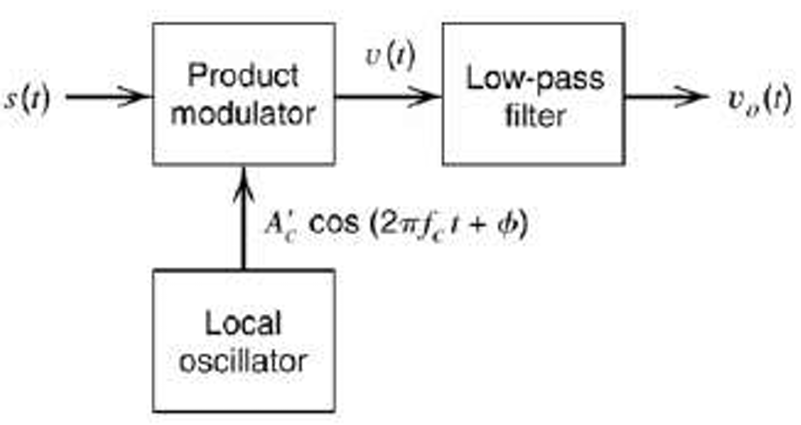
\includegraphics[width=0.6\textwidth]{fig2.png}
    \caption{Detector coherente}
    \label{fig:2}
\end{figure}
